\documentclass[10pt]{article}

\usepackage[letterpaper,left=2cm,right=2cm,top=1cm,bottom=1.25cm]{geometry}
\usepackage[T1]{fontenc}
\usepackage{lmodern}
\usepackage{microtype}
\usepackage{amsmath,amssymb,mathtools,bm}
\usepackage{authblk}
\usepackage{booktabs,tabularx,longtable,array,multirow}
\usepackage{graphicx,float,caption,subcaption}
\usepackage{enumitem}
\usepackage{xcolor}
\usepackage[most]{tcolorbox}
\usepackage[numbers,sort&compress]{natbib}
\usepackage{seqsplit}
\usepackage{url}
\usepackage{hyperref}
\usepackage{fancyhdr}

\definecolor{linkred}{RGB}{170,25,25}
\hypersetup{
  colorlinks=true,
  citecolor=linkred,
  urlcolor=linkred,
  linkcolor=black,
  pdfauthor={Dhruv Sharma},
  pdftitle={FDT-N: Footprint Distribution Transformer--Narrow. Inputs, Architecture, and Direct Multi-Horizon Quantile Outputs},
  pdfsubject={Research manuscript},
  pdfkeywords={volume footprint, transformer, marginal quantile forecasting, ragged attention, market microstructure}
}
\urlstyle{same}

\renewcommand\Authfont{\normalsize}
\renewcommand\Affilfont{\small\itshape}
\setlength{\affilsep}{0.35em}
\setlength{\parindent}{1.35em}
\setlength{\parskip}{0pt}
\setlength{\textfloatsep}{9pt plus 2pt minus 2pt}
\setlength{\floatsep}{8pt plus 2pt minus 2pt}
\setlist{nosep,leftmargin=1.8em}
\captionsetup{font=small,labelfont=bf}
\renewcommand{\arraystretch}{1.12}

\newcommand{\R}{\mathbb{R}}
\newcommand{\ind}{\mathbf{1}}
\newcommand{\softplus}{\operatorname{softplus}}
\newcommand{\RMSNorm}{\operatorname{RMSNorm}}
\newcommand{\MHA}{\operatorname{MHA}}
\newcommand{\clip}{\operatorname{clip}}
\newcommand{\sigmoid}{\operatorname{sigmoid}}
\newcommand{\hash}[1]{\texttt{\scriptsize\seqsplit{#1}}}
\newcommand{\qten}{q10}
\newcommand{\qfifty}{q50}
\newcommand{\qninety}{q90}

\pagestyle{fancy}
\fancyhf{}
\fancyhead[L]{\footnotesize FDT-N}
\fancyhead[R]{\footnotesize Dhruv Sharma}
\fancyfoot[C]{\thepage}
\setlength{\headheight}{13pt}

\newtcolorbox{definitionbox}[1]{
  enhanced,breakable,colback=black!3,colframe=black!70,
  boxrule=0.65pt,arc=0pt,left=6pt,right=6pt,top=5pt,bottom=5pt,
  title=\textbf{#1},coltitle=black,fonttitle=\normalsize,
  attach boxed title to top left={xshift=5pt,yshift=-2mm},
  boxed title style={colback=white,colframe=white,boxrule=0pt}
}
\newtcolorbox{evidencebox}[1]{
  enhanced,breakable,colback=blue!3,colframe=black!65,
  boxrule=0.65pt,arc=0pt,left=6pt,right=6pt,top=5pt,bottom=5pt,
  title=\textbf{#1},coltitle=black,fonttitle=\normalsize,
  attach boxed title to top left={xshift=5pt,yshift=-2mm},
  boxed title style={colback=white,colframe=white,boxrule=0pt}
}

\title{\vspace{-0.8em}\bfseries FDT-N: Footprint Distribution Transformer--Narrow\\[0.2em]
\large Inputs, Architecture, and Direct Multi-Horizon Quantile Outputs}
\author{Dhruv Sharma}
\affil{Independent Researcher}
\date{August 8, 2026}

\begin{document}
\maketitle
\vspace{-1.5em}

\begin{abstract}
\noindent Volume-footprint bars are variable-size sets of executed-volume rows. Footprint Distribution
Transformer--Narrow (FDT-N) maps a 64-bar ragged history to direct one- through eight-minute marginal
quantile forecasts. Its exported graph accepts four tensors: 11 features per price row, a row mask,
23 engineered features per bar, and a bar mask. Independent row embeddings feed four-query masked pooling; a
gate combines each row-set summary with its aggregate token; three causal temporal blocks encode the
history; and two decoder blocks process eight learned horizon queries. The 371,861-parameter model
returns $[B,8,7,3]$: batch, horizon, target, and q10/q50/q90. Targets are total POC, low, high, buy POC,
sell POC, relative log volume, and delta fraction. Softplus spreads order the marginal quantiles;
deterministic maps impose price-range relations and bound delta fraction.

The development corpus contains 20,160 one-minute BTCUSDT spot bars, 357,676 accepted rows, and 20,089
continuous 64+8 windows from January 1--14, 2024. A purged chronological split yields 13,990 training,
2,869 validation, and 2,942 test windows. Across three seeds, test pinball loss is
$0.07039$--$0.07154$ and q50 mean absolute error is $0.23587$--$0.23724$. For the selected seed, q50
error is 0.235870, versus 0.254298 for causal persistence and 0.229719 for train-only direct ridge;
central-80\% marginal coverage is 78.98\%. PyTorch and ONNX Runtime agree to maximum absolute error
$2.3842\times10^{-7}$ on the artifact-bound example.
\end{abstract}

\noindent\textbf{Keywords:} volume footprint; ragged sets; transformer; marginal quantile regression;
multi-horizon forecasting; market microstructure.

\section{Introduction}

A volume-footprint bar records executed buy- and sell-initiated volume at each traded price. Unlike
a conventional open-high-low-close-volume vector, the number of rows varies with the realized price
range. A model must therefore combine two structures: an order-invariant set stored in canonical
order and an ordered sequence of completed bars. Collapsing the rows to a few
aggregates is computationally convenient, but may erase distributional shape. Padding all bars to a
large fixed grid preserves more detail but wastes computation and makes overflow behavior easy to
hide.

FDT-N is a small hierarchical transformer designed around this representation mismatch. It uses
learned queries to reduce each variable-size row set to a fixed-width token and then models 64
completed-history tokens with a triangular attention mask. A parallel decoder produces eight horizons without feeding earlier forecasts
back into later ones. The output layer enforces within-target quantile order and elementary price
relationships. The final trained model contains 371,861 parameters.

``Narrow'' names this fixed compact configuration: width 64, four attention heads, three temporal
blocks, two decoder blocks, and 371,861 trainable parameters. It distinguishes the reported artifact
from a broader family of possible footprint transformers.

This paper answers two implementation questions directly: what tensors enter FDT-N, and what tensor
does it return? It then reports a chronological development benchmark against causal persistence and
train-only direct ridge. The selected FDT-N q50 has lower pooled error than persistence, while ridge
has the lowest pooled q50 error in this comparison. Those measurements characterize this corpus and
split; the architectural specification stands independently of comparator rank.

This paper makes four bounded contributions:

\begin{enumerate}
  \item It specifies the four-input ONNX contract, tensor shapes, axis order, dtypes, dynamic axes,
  chronological order, preprocessing boundary, and explicit 1,024-row acceptance bound.
  \item It derives learned-query row pooling, gated fusion, cutoff-causal temporal processing, the
  parallel horizon decoder, ordered marginal quantiles, physical constraints, and weighted pinball objective.
  \item It reports a hash-bound 14-day development experiment with three seeds, causal persistence,
  train-only direct ridge, per-target and per-horizon results, descriptive paired block resampling,
  export parity, and CPU timing.
  \item It traces one artifact-bound window from the four input tensors through named intermediate
  tensors to normalized and physical output values, with PyTorch--ONNX parity.
\end{enumerate}

\section{FDT-N at a glance: inputs, processing, and outputs}

\begin{figure}[H]
\centering
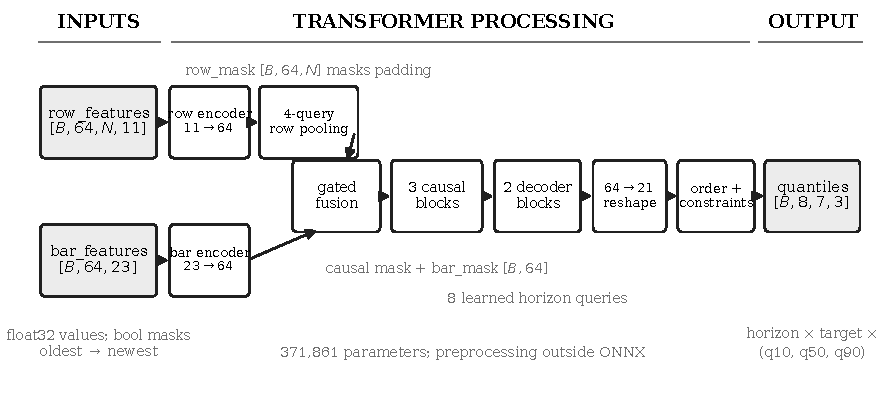
\includegraphics[width=\textwidth]{assets/architecture.pdf}
\caption{The complete FDT-N interface and forward path. Preprocessing produces four input tensors;
masked row pooling and temporal/decoder attention transform them; ordered and physically constrained
marginal quantiles form the single output tensor.}
\label{fig:architecture}
\end{figure}

\begin{table}[H]
\centering
\small
\caption{Exported ONNX interface. $B$ is dynamic batch size and $N$ is the dynamic batch-local row
width. Time runs oldest to newest. Preprocessing and inverse physical transforms are outside ONNX.}
\label{tab:io-contract}
\begin{tabularx}{\textwidth}{@{}l l l X@{}}
\toprule
Name & Type & Shape & Meaning / axis order \\
\midrule
\texttt{row\_features} & float32 & $[B,64,N,11]$ & eleven encoded features for every stored row \\
\texttt{row\_mask} & bool & $[B,64,N]$ & true exactly where a row is observed \\
\texttt{bar\_features} & float32 & $[B,64,23]$ & engineered bar/context features per completed bar \\
\texttt{bar\_mask} & bool & $[B,64]$ & true exactly where a history token is valid \\
\texttt{quantiles} & float32 & $[B,8,7,3]$ & horizon, target, quantile; target order
POC/low/high/buy-POC/sell-POC/log-volume/delta and quantile order .1/.5/.9 \\
\bottomrule
\end{tabularx}
\end{table}

For a batch of histories, the implemented forward map is
\begin{equation}
(X,M_R,F,M_B)\longmapsto E\longmapsto A\longmapsto U\longmapsto H
\longmapsto D\longmapsto R\longmapsto Q,
\label{eq:overview-map}
\end{equation}
with shapes
\begin{equation}
\begin{aligned}
X&:[B,64,N,11],& E&:[B,64,N,64],& A&:[B,64,64],\\
F&:[B,64,23],& U,H&:[B,64,64],& D&:[B,8,64],\\
R&:[B,8,7,3],& Q&:[B,8,7,3].
\end{aligned}
\label{eq:shape-trace}
\end{equation}
$M_R$ masks padded rows and $M_B$ masks padded history positions. $R$ stores the raw
$(c,s^-,s^+)$ head values; softplus ordering and target constraints convert it to $Q$. The returned
price and log-volume values are continuous normalized coordinates and may extend beyond the clipped
label range. Price inverse transforms can therefore lie between footprint-grid rows unless a consumer
applies a separately specified snapping policy. Buy- and sell-POC outputs are conditional on the
corresponding side being present in training labels; FDT-N emits no side-presence probability.

\begin{table}[H]
\centering
\small
\caption{Final architecture and exact trainable-parameter accounting.}
\label{tab:model-config}
\begin{tabular}{@{}lr@{}}
\toprule
Component / property & Value \\
\midrule
Row encoder, four-query pooling, row summary & 63,488 \\
Bar projection and gated residual fusion & 22,272 \\
Three temporal encoder blocks & 166,784 \\
Two-block eight-query horizon decoder & 117,888 \\
Output RMSNorm and $64\rightarrow21$ head & 1,429 \\
\midrule
Total trainable parameters & 371,861 \\
Model width / heads / head width & 64 / 4 / 16 \\
Dropout / initial LayerScale & 0.10 / $10^{-2}$ \\
\bottomrule
\end{tabular}
\end{table}

\section{Related work}

\subsection{Sets, attention, and ragged observations}

Deep Sets establishes a general permutation-invariant form based on elementwise representation and
symmetric aggregation \citep{zaheer2017deepsets}. Set Transformer replaces fixed summation with
attention-based interactions and learned inducing or seed vectors \citep{lee2019settransformer}.
Perceiver similarly uses a small latent array to query large inputs \citep{jaegle2021perceiver}.
FDT-N adopts the narrowest transferable idea: a constant number of learned queries cross-attends to
the observed rows. It does not use row-to-row self-attention, iterative latent refinement, or a claim
that attention weights explain market behavior \citep{jain2019attention}.

\subsection{Multi-horizon forecasting}

Temporal Fusion Transformer combines recurrent processing, gating, attention, and covariate
selection for multi-horizon probabilistic prediction \citep{lim2021tft}. PatchTST tokenizes temporal
patches \citep{nie2023patchtst}; iTransformer treats variables as tokens \citep{liu2024itransformer};
and Moirai studies universal time-series pretraining \citep{woo2024moirai}. DLinear demonstrates that
simple linear models can be informative forecasting controls \citep{zeng2023dlinear}. Accordingly,
direct ridge supplies a scale reference for FDT-N's q50 output. FDT-N is a task-specific 64-token
model rather than a foundation model.

\subsection{Market microstructure}

DeepLOB applies convolutional and recurrent layers to fixed-depth limit-order-book states
\citep{zhang2019deeplob}. FI-2010 provides a benchmark for mid-price prediction from limit-order-book
data \citep{ntakaris2018benchmark}; later work studies transformers and multi-horizon order-flow
imbalance \citep{wallbridge2020transformers,kolm2023orderflow}. A footprint is different from a book:
it summarizes executed trades by price inside a completed interval, whereas a limit-order-book tensor
describes displayed resting liquidity. Results do not transfer automatically between the two.

\subsection{Probabilistic prediction under dependence}

Quantile regression uses asymmetric absolute loss to estimate conditional quantiles
\citep{koenker1978quantile}, and proper scoring rules provide a principled basis for probabilistic
evaluation \citep{gneiting2007probabilistic}. Noncrossing constraints can be estimated or imposed by
parameterization \citep{bondell2010noncrossing}. Conformalized quantile regression can adjust
intervals under a separate calibration design and stated assumptions \citep{romano2019cqr}; this
study has no such partition. Because adjacent forecast windows overlap, we use paired contiguous
block resampling inspired by dependent-data bootstrap methods \citep{kunsch1989bootstrap}. We do not
present it as an independent-block confidence interval or a Diebold--Mariano test
\citep{diebold1995predictive}.

\section{Volume-footprint representation}

\subsection{Executed-volume rows}

For price row $j$ in completed bar $t$, define
\begin{equation}
r_{t,j}=\bigl(p_{t,j},v^+_{t,j},v^-_{t,j},I^{bid}_{t,j},I^{ask}_{t,j},
z^{bid}_{t,j},z^{ask}_{t,j}\bigr),
\end{equation}
where $p$ is the snapped row price, $v^+$ is buy-initiated (ask-lifting) volume, $v^-$ is
sell-initiated (bid-hitting) volume, $I$ are diagonal-imbalance flags, and $z$ are explicit zero-side
flags. Total executed volume and signed delta at the row are
\begin{equation}
v_{t,j}=v^+_{t,j}+v^-_{t,j},\qquad
\Delta_{t,j}=v^+_{t,j}-v^-_{t,j}.
\label{eq:row-total-delta}
\end{equation}
Adding and subtracting these two equations gives the inverse identities
\begin{equation}
v^+_{t,j}=\frac{v_{t,j}+\Delta_{t,j}}{2},\qquad
v^-_{t,j}=\frac{v_{t,j}-\Delta_{t,j}}{2}.
\label{eq:row-inverse}
\end{equation}
Since both side volumes are nonnegative, $v+\Delta\ge0$ and $v-\Delta\ge0$; therefore
\begin{equation}
-v_{t,j}\le\Delta_{t,j}\le v_{t,j},\qquad |\Delta_{t,j}|\le v_{t,j}.
\end{equation}
This is an accounting constraint, not a directional trading rule. Positive delta only says that
aggressive buy volume exceeded aggressive sell volume at that row.

For imbalance ratio $\lambda$ (3 by default), the stored diagonal flags compare opposite sides at
adjacent prices:
\begin{equation}
I^{bid}_{t,j}=\ind\!\left[v^-_{t,j}>0\ \land\ v^-_{t,j}\ge\lambda v^+_{t,j-1}\right],\qquad
I^{ask}_{t,j}=\ind\!\left[v^+_{t,j}>0\ \land\ v^+_{t,j}\ge\lambda v^-_{t,j+1}\right].
\end{equation}
The exact neighbor direction follows the high-to-low row ordering; a missing outer neighbor has
volume zero. The flags record a thresholded relationship; they do not preserve the underlying ratio.

\subsection{From rows to bar statistics}

Let $R_t=\{r_{t,1},\ldots,r_{t,n_t}\}$ contain every accepted row of bar $t$. Side, total, and delta
volumes are additive:
\begin{equation}
V_t^+=\sum_{j=1}^{n_t}v^+_{t,j},\quad
V_t^-=\sum_{j=1}^{n_t}v^-_{t,j},\quad
V_t=V_t^++V_t^-,\quad
\Delta_t=V_t^+-V_t^-.
\label{eq:bar-volumes}
\end{equation}
The point of control (POC) is a mode, not an average:
\begin{equation}
j_t^*=\arg\max_j v_{t,j},\qquad p_t^{POC}=p_{t,j_t^*}.
\label{eq:poc}
\end{equation}
Buy and sell POCs replace $v_{t,j}$ in Eq.~\eqref{eq:poc} by $v^+_{t,j}$ and $v^-_{t,j}$.
Rows are sorted from high to low, and ties resolve to the first maximum, hence the highest price.
For an all-zero side, this argmax still returns the highest observed row, but the corresponding future
side-POC target is masked. By contrast, the volume centroids are weighted means:
\begin{equation}
c_t=\frac{\sum_j p_{t,j}v_{t,j}}{V_t},\quad
c_t^+=\frac{\sum_j p_{t,j}v^+_{t,j}}{V_t^+}\ (V_t^+>0),\quad
c_t^-=\frac{\sum_j p_{t,j}v^-_{t,j}}{V_t^-}\ (V_t^->0).
\label{eq:centroids}
\end{equation}
A POC answers ``where was the most volume at one row?''; a centroid answers ``where was the average
unit of volume?'' They coincide only in special cases. A side centroid is mathematically undefined
when that side has zero volume; the implemented FDT preprocessing fills its fixed input slot with the
total-POC price. The future side-POC target is masked whenever its side volume is zero.

For target fraction $\eta=0.70$, the value area is a deterministic contiguous interval around the
total POC. Let $[\ell_m,u_m]$ be the current high-to-low index interval, initialized at
$\ell_0=u_0=j_t^*$. Define the available volume immediately above and below as
\begin{equation}
a_m=\begin{cases}v_{t,\ell_m-1},&\ell_m>1,\\-1,&\text{otherwise},\end{cases}
\qquad
b_m=\begin{cases}v_{t,u_m+1},&u_m<n_t,\\-1,&\text{otherwise}.
\end{cases}
\end{equation}
If $b_m>a_m$, set $u_{m+1}=u_m+1$; otherwise set $\ell_{m+1}=\ell_m-1$, leaving the other bound
unchanged. Thus an equal-volume tie expands upward to the higher price. Continue until
\begin{equation}
\frac{\sum_{j=\ell_m}^{u_m}v_{t,j}}{V_t}\ge\eta.
\end{equation}
The final lowest and highest prices are value-area low and high. Contiguity makes this different from
selecting the globally largest 70\% of rows. Bar high and low are the extreme observed row prices.
Cumulative volume delta obeys
\begin{equation}
CVD_t=CVD_{t-1}+\Delta_t,
\end{equation}
so its reset policy is part of the coordinate definition. In this corpus, CVD starts at zero at the
beginning of the 14-day build and carries across sealed bars. Feature 15 later subtracts the first
context CVD, making it invariant to an additive global reset within the encoded series.

\begin{definitionbox}{Causal availability}
A bar is usable only after its interval has ended and the configured feed-completeness decision is
available. No event, normalization statistic, model-selection choice, or calibration value whose
availability follows the forecast cutoff may affect the input. Event time alone is insufficient when
late data can arrive.
\end{definitionbox}

\section{Input construction and forecasting task}

\subsection{Information set and direct horizons}

Let $B_t=(R_t,b_t)$ denote the row set and engineered bar/context features of completed bar $t$.
For lookback $L=64$ and horizon count $H=8$, the forecast map is
\begin{equation}
\widehat{Y}_{t+1:t+H}=F_\theta\!\left(B_{t-L+1:t}\right),
\qquad
\widehat{Y}\in\R^{H\times K\times Q},
\label{eq:forecast-map}
\end{equation}
with $K=7$ targets and $Q=3$ quantile levels $\mathcal T=\{0.1,0.5,0.9\}$.
The information set ends at the seal of $B_t$. Every adjacent timestamp across the 64 input bars and
8 label bars must differ by exactly 60 seconds. Thus a candidate starting at $s$ is valid only if
\begin{equation}
T_{i+1}-T_i=60\ \mathrm{seconds}\quad
\text{for every }i=s,\ldots,s+L+H-2.
\label{eq:continuity}
\end{equation}
Missing or irregular intervals invalidate the window; they are not treated as adjacent market time.

The model is direct: all eight outputs are functions of the same historical information set,
\begin{equation}
(\widehat Y_1,\ldots,\widehat Y_8)=F_\theta(B_{t-63:t}),
\end{equation}
rather than an autoregression $\widehat Y_h=f(B_{t-63:t},\widehat Y_{1:h-1})$. This distinction
removes forecast-as-input error propagation but does not make errors across horizons independent.

\subsection{Ragged storage and masks}

Row counts $n_t$ vary by bar. The encoded series therefore concatenates rows into one matrix
$E\in\R^{N\times 11}$ and stores offsets $o_0=0$ and
\begin{equation}
o_{t+1}=o_t+n_t,\qquad R_t\longleftrightarrow E[o_t:o_{t+1},:].
\label{eq:ragged-offset}
\end{equation}
Within a window, shorter bars are padded to the widest observed local row count; batching may then pad
windows to the batch-local maximum. A binary mask $m_{t,j}$ equals 1 for observed rows and 0 for
padding. In attention logits, padding receives $-\infty$, so its softmax weight is exactly zero in
ideal arithmetic. Batches are limited by both item count and padded row-width budget; wide windows
produce smaller batches rather than dropped rows. The export keeps the row axis dynamic.

The accepted-row contract is $n_t\le1{,}024$; a bar outside that domain is not encoded. Every row is
retained for accepted bars. In the frozen corpus, the maximum is 605.

\subsection{Input coordinates}

Let $\delta_p=2.5$ USDT be the footprint-row size and let
$\kappa(p)=p/\delta_p$ denote the integer row coordinate after snapping. Accepted bars satisfy
$V_t>0$. For each row, define $S_g=32$ row increments. The implemented 11-vector is
\begin{align}
x_{t,j}^{(1)}&=\clip\!\left(\frac{\kappa(p_{t,j})-\kappa(p_t^{POC})}{S_g},-2,2\right),\\
x_{t,j}^{(2:4)}&=\left(\frac{v^+_{t,j}}{V_t},\frac{v^-_{t,j}}{V_t},
\frac{v_{t,j}}{V_t}\right),\\
x_{t,j}^{(5)}&=\frac{\Delta_{t,j}}{V_t},\\
x_{t,j}^{(6:7)}&=\left(\frac{\log(1+v^+_{t,j})}{\log(1+V_t)},
\frac{\log(1+v^-_{t,j})}{\log(1+V_t)}\right),\\
x_{t,j}^{(8:11)}&=(I^{bid}_{t,j},I^{ask}_{t,j},z^{bid}_{t,j},z^{ask}_{t,j}).
\label{eq:row-features}
\end{align}
When $V_t>0$, the side shares sum to the total share, and summing the total share across rows gives 1.
The logarithmic ratios compress scale while retaining zeros. The binary flags remain discrete facts.

The 23-dimensional bar vector is separately projected. Table~\ref{tab:bar-features} states its
schema order; reordering it would change the model coordinate.

\begin{table}[H]
\centering
\small
\caption{Implemented aggregate bar features in schema order. All price quantities are normalized
row-coordinate offsets; references are computed from context only.}
\label{tab:bar-features}
\begin{tabularx}{\textwidth}{@{}c l X@{}}
\toprule
Index & Feature(s) & Meaning \\
\midrule
1 & POC offset & total POC relative to the last-context anchor POC \\
2--3 & buy/sell POC offsets & side POCs relative to the bar POC \\
4--6 & total/buy/sell centroid offsets & Eq.~\eqref{eq:centroids} relative to the bar POC \\
7--10 & low, high, value-area gaps & lower and upper structure around the bar POC \\
11 & relative log volume & log volume relative to a context-only median \\
12--14 & buy, sell, delta fractions & $V^+/V$, $V^-/V$, and $\Delta/V$ \\
15 & cumulative-delta change & context-relative CVD change, scaled by 4 \\
16--17 & stacked buy/sell fractions & normalized run-length summaries \\
18 & row-count fraction & log-scaled row count under the 1,024-row bound \\
19 & feed quality & raw source-quality scalar (1.0 in this corpus) \\
20--23 & calendar cycle & sine/cosine of minute-of-day and weekday \\
\bottomrule
\end{tabularx}
\end{table}

The exact aggregate transform follows. Express prices as row ticks and write, for context bar $r$,
$P_r$ for total POC; $P_r^+,P_r^-$ for side POCs; $C_r,C_r^+,C_r^-$ for centroids; $L_r,H_r$ for
low/high; $A_r^L,A_r^H$ for value-area bounds; $D_r$ for CVD; $S_r^+,S_r^-$ for stacked-run lengths;
and $n_r$ for row count. The context-only references are
\begin{equation}
P^*=P_t,\qquad
\widetilde\ell_t=\operatorname{median}\{\log(1+V_r):r=t-15,\ldots,t\},\qquad
V^*=\exp(\widetilde\ell_t)-1,\qquad D_0=D_{t-L+1}.
\label{eq:volume-reference}
\end{equation}
For $S_p=64$, $S_g=32$, $S_v=S_c=4$, and $n_{max}=1024$, features 1--15 are
\begin{align}
f_{r,1}&=\clip((P_r-P^*)/S_p,-2,2),\\
(f_{r,2},f_{r,3})&=\bigl(\clip((P_r^+-P_r)/S_g,-2,2),
\clip((P_r^--P_r)/S_g,-2,2)\bigr),\\
(f_{r,4},f_{r,5},f_{r,6})&=\bigl(\clip((C_r-P_r)/S_g,-2,2),
\clip((C_r^+-P_r)/S_g,-2,2),\clip((C_r^--P_r)/S_g,-2,2)\bigr),\\
(f_{r,7},f_{r,8})&=\bigl(\min((P_r-L_r)/S_g,2),
\min((H_r-P_r)/S_g,2)\bigr),\\
(f_{r,9},f_{r,10})&=\bigl(\min((P_r-A_r^L)/S_g,2),
\min((A_r^H-P_r)/S_g,2)\bigr),\\
f_{r,11}&=\clip((\log(1+V_r)-\widetilde\ell_t)/S_v,-2,2),\\
(f_{r,12},f_{r,13},f_{r,14})&=\left(V_r^+/V_r,V_r^-/V_r,
(V_r^+-V_r^-)/V_r\right),\\
f_{r,15}&=\clip\!\left(\frac{D_r-D_0}{S_c\max(V^*L,1)},-2,2\right).
\label{eq:bar-features-exact}
\end{align}
The structural gaps in features 7--10 are expected nonnegative, so the implementation caps only the
upper side. The remaining features are
\begin{align}
f_{r,16}&=\min(S_r^+/\max(n_r,1),1),&
f_{r,17}&=\min(S_r^-/\max(n_r,1),1),\\
f_{r,18}&=\min\!\left(\frac{\log(1+n_r)}{\log(1+n_{max})},1\right),&
f_{r,19}&=q_r,\\
f_{r,20:21}&=\left(\sin(2\pi m_r/1440),\cos(2\pi m_r/1440)\right),\\
f_{r,22:23}&=\left(\sin(2\pi w_r/7),\cos(2\pi w_r/7)\right).
\end{align}
For bar-start time $T_r$ in Unix milliseconds,
$m_r=(\lfloor T_r/60000\rfloor\bmod1440)$ and
$w_r=(\lfloor T_r/86400000\rfloor+3)\bmod7$, with Monday equal to zero. $q_r$ is the raw quality
field; it is 1.0 throughout this frozen Binance corpus. Every reference in
Eqs.~\eqref{eq:volume-reference}--\eqref{eq:bar-features-exact} is constructed only from archive
events assigned to bars ending by the final event-time cutoff, even though an early token uses
context-wide reference constants as discussed in Section~\ref{sec:temporal}.
Section~\ref{sec:scope} summarizes the distinction between event-time reconstruction and live
receive-time availability.

\subsection{Targets and inverse transforms}

Let $\mathcal P=\{POC,low,high,buyPOC,sellPOC\}$, $S_p=64$ row increments, and $S_v=4$. For future
horizon $h$ and price target $k\in\mathcal P$,
\begin{equation}
y_h^k=\clip\!\left(
\frac{\kappa(p_{t+h}^k)-\kappa(p_t^{POC})}{S_p},-2,2\right).
\label{eq:price-target}
\end{equation}
Low, high, and side POCs are direct offsets from the cutoff anchor; they are not gaps from an unknown
future POC. The remaining targets are
\begin{align}
y_h^V&=\clip\!\left(
\frac{\log(1+V_{t+h})-\widetilde\ell_t}{S_v},-2,2\right),
\label{eq:volume-target}\\
y_h^\Delta&=\clip\!\left(
\frac{V^+_{t+h}-V^-_{t+h}}{V^+_{t+h}+V^-_{t+h}},-1,1\right).
\label{eq:delta-target}
\end{align}
Buy- and sell-POC labels are masked independently if the relevant side volume is absent.

Ignoring clipping for the moment, a normalized price quantile $q_h^k$ maps back to physical price as
\begin{equation}
\widehat p_{t+h,\tau}^k=p_t^{POC}+\delta_p S_p\widehat q_{h,k,\tau},
\end{equation}
and a normalized volume quantile maps to
\begin{equation}
\widehat V_{t+h,\tau}=\exp\!\left(\widetilde\ell_t+S_v\widehat q_{h,V,\tau}\right)-1.
\end{equation}
The volume inverse is nonnegative exactly when
$\widetilde\ell_t+S_v\widehat q_{h,V,\tau}\ge0$. Price and log-volume heads are continuous and
unbounded even though training labels are clipped; delta fraction is bounded by $\tanh$. Consumers
can retain normalized coordinates or define a domain policy for physical values. Each inverse is
marginal: applying it separately to the seven targets does not construct a joint future candle.

\subsection{Frozen development corpus and split}

The data comprise official Binance Data Vision BTCUSDT spot individual-trade archives
\citep{binance2024datavision} for January 1--14, 2024. For trade event time $T$ in milliseconds, bar
start is $T-(T\bmod60000)$. A positive price is snapped to tick
$\lfloor p/2.5+0.5\rfloor$. A trade is buy-initiated when Binance's
\texttt{buyer\_is\_maker} flag is false and sell-initiated when it is true. Quantity is multiplied by
1,000, rounded with Python's ties-to-even \texttt{round} semantics, converted to integer, and dropped
when the result is nonpositive. The same coordinate is used by the extractor and model package.

\begin{table}[H]
\centering
\small
\caption{Frozen development-corpus and chronological-split facts.}
\label{tab:corpus}
\begin{tabular}{@{}lr@{}}
\toprule
Item & Value \\
\midrule
Venue / instrument / source & Binance spot BTCUSDT individual trades \\
UTC span & 2024-01-01 00:00 through 2024-01-14 23:59 \\
Bar interval / footprint row size & 60 seconds / 2.5 USDT \\
Completed bars / complete accepted rows & 20,160 / 357,676 \\
Rows per bar, p50 / p95 / p99 / maximum & 13 / 47 / 94.41 / 605 \\
Valid continuous 64+8 windows & 20,089 \\
Train / validation / test windows & 13,990 / 2,869 / 2,942 \\
Purge around each split boundary & 72 window starts per side; 144 per boundary \\
Test-context span & 2024-01-12 22:50 through 2024-01-14 23:51 UTC \\
Calibration partition / untouched outer holdout & none / none \\
\bottomrule
\end{tabular}
\end{table}

Table~\ref{tab:corpus} fixes the venue, period, row grid, corpus size, and split counts used below.
The archives support event-time reconstruction but do not preserve the original live receive time,
availability decision, or late-arrival acceptance epoch. Accordingly, Eq.~\eqref{eq:continuity} and
the split establish mechanical event-time cutoff separation, not a verified historical simulation of
when every trade would have been available online. The submission bundle's lineage record begins at
the official archives and preserves the encoded counts. These statements characterize data lineage
rather than forecast output.

\begin{figure}[H]
\centering
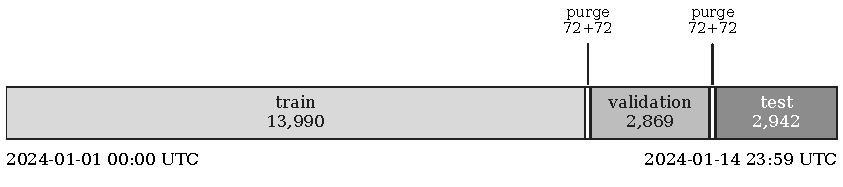
\includegraphics[width=0.98\textwidth]{assets/split-timeline.pdf}
\caption{Chronological development split. At each boundary, 72 window starts are removed from each
adjacent partition, giving 144 removed starts per boundary and 288 in total. The figure widths are
proportional to the 20,089 valid window starts.}
\label{fig:split}
\end{figure}

Figure~\ref{fig:split} visualizes the chronological partitions and the two purged boundaries.
A window consumes $L$ context bars and $H$ label bars, a span of $L+H=72$ bar indices. Without a
purge, a training label interval could overlap a validation context or label interval. The split
removes 72 candidate window starts on both sides of each of the two boundaries: $4\times72=288$
starts. The identity $13{,}990+2{,}869+2{,}942+288=20{,}089$ reconciles the reported counts. This
conservative separation leaves serial dependence within each partition; a later outer period is part
of the follow-up design in Section~\ref{sec:follow-up}.

\section{Transformer processing pipeline}

Figure~\ref{fig:architecture} and Eq.~\eqref{eq:shape-trace} give the complete path. This section
defines each learned transformation, including normalization, residual paths, masks, and dimensions.

\subsection{Independent row encoder}

For a bar with $n_t$ rows, stack the features from Eq.~\eqref{eq:row-features} into
$X_t\in\R^{n_t\times11}$. The same two-layer map is applied independently to each row:
\begin{equation}
e_{t,j}=\RMSNorm\!\left(W_2\,\operatorname{GELU}(W_1x_{t,j}+b_1)+b_2\right)
\in\R^d.
\label{eq:row-mlp}
\end{equation}
Here $W_1\in\R^{64\times11}$ and $W_2\in\R^{64\times64}$, so the width is
$11\rightarrow64\rightarrow64$. GELU is $z\Phi(z)$ \citep{hendrycks2016gelu}.

For $u\in\R^d$, RMSNorm is
\begin{equation}
\RMSNorm(u)=g\odot\frac{u}{\sqrt{d^{-1}\sum_{i=1}^d u_i^2+\epsilon}},
\label{eq:rmsnorm}
\end{equation}
with learned scale $g$ \citep{zhang2019rmsnorm}. RMSNorm rescales without mean subtraction. At this
stage no row has interacted with another row; mixing occurs only in query pooling.

\subsection{Learned-query multi-head row pooling}

Let $K_q=4$ learned query vectors form $Q_0\in\R^{K_q\times d}$. The implemented cross-attention
block first normalizes queries and row memory independently:
\begin{align}
\bar Q_0&=\RMSNorm_Q(Q_0),& \bar E_t&=\RMSNorm_M(E_t),\\
C_t&=Q_0+\operatorname{Drop}_{.1}\!\left(\MHA(\bar Q_0,\bar E_t,\bar E_t;M_t)\right),\\
O_t&=C_t+\operatorname{Drop}_{.1}\!\left(
\operatorname{SwiGLU}_{128}(\RMSNorm_F(C_t))\right).
\label{eq:row-cross-block}
\end{align}
For attention head $a$ with $d_h=d/A=16$,
\begin{align}
Q^{(a)}&=\bar Q_0W_Q^{(a)}\in\R^{K_q\times d_h},\\
K_t^{(a)}&=\bar E_tW_K^{(a)}\in\R^{n_t\times d_h},\\
V_t^{(a)}&=\bar E_tW_V^{(a)}\in\R^{n_t\times d_h},
\end{align}
where $E_t$ stacks the row embeddings. Scores, weights, and pooled outputs are
\begin{align}
S_t^{(a)}&=\frac{Q^{(a)}K_t^{(a)\top}}{\sqrt{d_h}}+M_t,
&&S_t^{(a)}\in\R^{K_q\times n_t},\\
A_t^{(a)}&=\operatorname{softmax}_{j}\!\left(S_t^{(a)}\right),\\
O_t^{(a)}&=A_t^{(a)}V_t^{(a)}\in\R^{K_q\times d_h}.
\label{eq:row-attention}
\end{align}
The $1/\sqrt{d_h}$ factor controls score scale: if independent query and key components have unit
variance, their dot product has variance $d_h$; division restores order-one variance
\citep{vaswani2017attention}. $M_{t,kj}=0$ for an observed row and $-\infty$ for padding. Concatenating
the four heads and projecting supplies the MHA value in Eq.~\eqref{eq:row-cross-block}. The resulting
four $64$-vectors are flattened and reduced by
\begin{equation}
a_t=\RMSNorm\!\left(\operatorname{GELU}(W_s\operatorname{vec}(O_t)+b_s)\right),
\qquad W_s\in\R^{64\times256}.
\label{eq:row-summary}
\end{equation}

\paragraph{Permutation-invariance derivation.}
Let $P$ be any $n_t\times n_t$ row-permutation matrix. Permuting rows changes keys and values to
$PK$ and $PV$. The new score matrix is $Q(PK)^\top=QK^\top P^\top$. Rowwise softmax commutes with
column permutation, so
\begin{equation}
\operatorname{softmax}(QK^\top P^\top)=\operatorname{softmax}(QK^\top)P^\top.
\end{equation}
Multiplying by $PV$ cancels the permutation:
\begin{equation}
\operatorname{softmax}(QK^\top)P^\top PV
=\operatorname{softmax}(QK^\top)V.
\end{equation}
Therefore query pooling is invariant to row order, provided the features and mask receive the same
permutation. The extractor still stores rows canonically for deterministic serialization.

The attention score term is $O(K_qn_td_h)$ per head, or $O(K_qn_td)$ across heads, instead of the
$O(n_t^2d)$ score term of row self-attention. Linear projections still cost $O(n_td^2)$. The four
queries provide four learned summary slots without assigning a fixed market semantic to any slot.

\subsection{Gated row/aggregate fusion}

Project the 23 bar features to $b_t\in\R^d$ and concatenate $z_t=[a_t;b_t]\in\R^{2d}$. Fusion is
\begin{align}
g_t&=\sigmoid(W_gz_t+b_g)\in(0,1)^d,
\label{eq:fusion-gate}\\
u_t&=g_t\odot a_t+(1-g_t)\odot b_t+W_rz_t+b_r.
\label{eq:fusion}
\end{align}
The bar projection is $23\rightarrow64\rightarrow64$ with GELU and RMSNorm. In
Eq.~\eqref{eq:fusion}, the first two terms interpolate coordinatewise, while $W_rz_t+b_r$ provides a
direct learned residual path from both summaries.

\subsection{Causally masked temporal encoder}
\label{sec:temporal}

Add row $i$ of a learned $64\times64$ time-embedding table to each fused token, producing
$H^{(0)}_i=u_{t-L+i}+p_i$ for $i=1,\ldots,L$. In each pre-normalized temporal block, masked
self-attention and a gated feed-forward network are applied with residual LayerScale:
\begin{align}
Z&=H+\gamma_A\odot\operatorname{Drop}_{.1}\!\left(
\MHA(\RMSNorm(H);M^{causal},M_B)\right),
\label{eq:temporal-attn}\\
H'&=Z+\gamma_F\odot\operatorname{Drop}_{.1}\!\left(
\operatorname{SwiGLU}_{192}(\RMSNorm(Z))\right).
\label{eq:temporal-ffn}
\end{align}
The learned vectors $\gamma_A,\gamma_F\in\R^d$ start at $10^{-2}$, limiting the initial residual
branch magnitude \citep{touvron2021layerscale}. For feed-forward width $d_f=3d$, SwiGLU is
\begin{equation}
\operatorname{SwiGLU}(x)=W_o\left[\operatorname{SiLU}(W_gx+b_g)\odot(W_ux+b_u)\right]+b_o,
\label{eq:swiglu}
\end{equation}
where $\operatorname{SiLU}(z)=z\sigmoid(z)$ \citep{shazeer2020glu}. $M_B$ excludes padded history
tokens as attention keys. After three blocks, a final RMSNorm produces memory
$\mathcal H\in\R^{B\times64\times64}$.

For temporal positions $i,j\in\{1,\ldots,L\}$,
\begin{equation}
M^{causal}_{ij}=\begin{cases}0,&j\le i,\\-\infty,&j>i.\end{cases}
\label{eq:causal-mask}
\end{equation}
At position $i$, every future logit is $-\infty$; its exponential is zero, so temporal attention
reads only positions $j\le i$. The common price anchor and volume reference in
Eqs.~\eqref{eq:volume-reference}--\eqref{eq:volume-target} are computed at the final cutoff from the
full 64-bar context, so an early token can indirectly encode information about later \emph{historical}
context bars through those shared coordinates. Every anchor, reference, and token is nevertheless
available at the forecast cutoff.

\subsection{Parallel horizon decoder}

For each horizon $h$, initialize a decoder token from two learned vectors,
\begin{equation}
D_h^{(0)}=q_h^{hor}+e_h^{hor}.
\end{equation}
Both learned tables have shape $8\times64$; their sum initializes the eight tokens rather than
representing two separately supervised concepts. Decoder block $\ell\in\{1,2\}$ first applies
unmasked self-attention among the eight horizon tokens, then cross-attention to the history, and then
a width-128 gated feed-forward sublayer:
\begin{align}
A^{(\ell)}&=D^{(\ell-1)}+\operatorname{Drop}_{.1}\!\left[
\MHA\!\left(\RMSNorm_S(D^{(\ell-1)})\right)\right],\\
C^{(\ell)}&=A^{(\ell)}+\operatorname{Drop}_{.1}\!\left[
\MHA\!\left(\RMSNorm_Q(A^{(\ell)}),
\RMSNorm_M(\mathcal H),\RMSNorm_M(\mathcal H);M_B\right)\right],\\
D^{(\ell)}&=C^{(\ell)}+\operatorname{Drop}_{.1}\!\left[
\operatorname{SwiGLU}_{128}(\RMSNorm_F(C^{(\ell)}))\right].
\label{eq:decoder-block}
\end{align}
The self-attention is unmasked because no token contains a realized target or earlier forecast. The
cross-attention uses four heads of width 16, with the decoder tokens as queries and the 64 historical
states as keys and values. Thus all eight outputs are direct functions of the same cutoff history.

\subsection{Output projection and in-graph constraints}

Final decoder normalization followed by one affine projection gives
\begin{equation}
R=\operatorname{reshape}_{8\times7\times3}\!\left(
W_o\RMSNorm_O(D^{(2)})+b_o\right),
\qquad W_o\in\R^{21\times64}.
\label{eq:output-head}
\end{equation}
The last axis of $R$ is $(c,s^-,s^+)$. Equations~\eqref{eq:ordered-quantiles} and
\eqref{eq:physical-constraints}, plus $\tanh$ for delta, execute inside the forward graph before
either the training loss or ONNX output is produced. The resulting $Q\in\R^{B\times8\times7\times3}$
is therefore the constrained tensor consumed by both training and inference.

\subsection{Complexity and tensor accounting}

With average row count $\bar n$, temporal depth $N_T=3$, decoder depth $N_D=2$, and fixed model width,
the principal attention-score complexity is
\begin{equation}
O(LK_q\bar n d)+O(N_TL^2d)+O(N_DHLd)+O(N_DH^2d).
\label{eq:complexity}
\end{equation}
The four terms are row-query pooling, temporal self-attention, history cross-attention, and horizon
self-attention. With $L=64$ and $H=8$, one temporal layer has only $64^2=4{,}096$ position pairs per
head. Peak row activation storage is proportional to the padded batch width rather than a global
1,024-row rectangle for every bar. The full shape trace and parameter subtotals appear in
Eq.~\eqref{eq:shape-trace} and Table~\ref{tab:model-config}.

\section{Outputs, physical constraints, and training objective}

\subsection{A noncrossing marginal parameterization}

For each horizon and target, the unconstrained head emits a center $c$ and two spread logits
$s^-,s^+$. Define
\begin{align}
\widetilde Q_{0.10}&=c-\softplus(s^-)-\epsilon_q,\\
\widetilde Q_{0.50}&=c,\\
\widetilde Q_{0.90}&=c+\softplus(s^+)+\epsilon_q,
\label{eq:ordered-quantiles}
\end{align}
where $\softplus(s)=\log(1+e^s)>0$ and $\epsilon_q=10^{-4}$. Therefore
\begin{equation}
\widetilde Q_{0.10}<\widetilde Q_{0.50}<\widetilde Q_{0.90}
\end{equation}
for every finite pair of spread logits. Differentiating gives
$d\softplus(s)/ds=\sigmoid(s)$, so spread gradients are smooth and bounded between 0 and 1. This
guarantees order; it does not guarantee that empirical exceedance frequencies equal 10\%, 50\%, and
90\%.

\subsection{Quantilewise price constraints}

All five price heads use the same anchor-relative coordinate. For a fixed $\tau$, let
$\widetilde L_\tau,\widetilde H_\tau,\widetilde P_\tau,
\widetilde B_\tau,\widetilde S_\tau$ denote unconstrained low, high, total-POC, buy-POC, and sell-POC
quantiles after Eq.~\eqref{eq:ordered-quantiles}. The implemented map is
\begin{align}
P_\tau&=\widetilde P_\tau,\\
L_\tau&=\min(\widetilde L_\tau,P_\tau),\\
H_\tau&=\max(\widetilde H_\tau,P_\tau),\\
B_\tau&=\min\!\left(\max(\widetilde B_\tau,L_\tau),H_\tau\right),\\
S_\tau&=\min\!\left(\max(\widetilde S_\tau,L_\tau),H_\tau\right).
\label{eq:physical-constraints}
\end{align}
It follows immediately that
\begin{equation}
L_\tau\le P_\tau,B_\tau,S_\tau\le H_\tau.
\end{equation}
Low and high expand only enough to include total POC; side POCs are clamped and do not expand the
range. The scalar functions $\min$ and $\max$ are coordinatewise monotone. Since every input sequence
in $\tau$ is ordered by Eq.~\eqref{eq:ordered-quantiles}, compositions in
Eq.~\eqref{eq:physical-constraints} preserve within-target order across $\tau$. Delta-fraction
quantiles pass through the monotone map $\tanh$, which preserves order while bounding them to
$[-1,1]$.

These relationships are necessary physical conditions, not a full probabilistic model. Quantilewise
constraints do not specify cross-target dependence, and $L_{0.10}$ together with $H_{0.90}$ is not a
guaranteed joint-candle interval.

\subsection{Pinball loss and its quantile derivation}

For observation $y$, forecast $q$, residual $e=y-q$, and quantile level $\tau\in(0,1)$, pinball loss is
\begin{equation}
\rho_\tau(e)=\max\{\tau e,(\tau-1)e\}
=\begin{cases}
\tau(y-q),&y\ge q,\\
(1-\tau)(q-y),&y<q.
\end{cases}
\label{eq:pinball}
\end{equation}
Thus underpredicting q90 costs $0.9$ per unit while overpredicting it costs $0.1$ per unit. To see why
the optimum is a conditional quantile, take expectation under conditional cumulative distribution
$F$. At a continuity point,
\begin{align}
R(q)&=\mathbb E[\rho_\tau(Y-q)]\\
&=(1-\tau)\int_{-\infty}^{q}(q-y)dF(y)
+\tau\int_q^\infty(y-q)dF(y),\\
\frac{dR(q)}{dq}&=(1-\tau)F(q)-\tau[1-F(q)]=F(q)-\tau.
\end{align}
Any stationary minimum therefore satisfies $F(q)=\tau$. With atoms, the subgradient condition is
$F(q^-)\le\tau\le F(q)$, which is precisely the definition of a valid $\tau$-quantile
\citep{koenker1978quantile}.

For batch item $b$, horizon $h$, target $k$, and level $\tau$, let $m_{bhk}\in\{0,1\}$ indicate a
valid label. The implemented objective is
\begin{equation}
\mathcal L=
\frac{\sum_{b,h,k,\tau}m_{bhk}w_hw_k
\rho_\tau(y_{bhk}-\widehat q_{bhk\tau})}
{\sum_{b,h,k,\tau}m_{bhk}w_hw_k},
\qquad w_h=\frac{1}{\sqrt h}.
\label{eq:weighted-loss}
\end{equation}
The target weights in schema order are
$(1.0,0.7,0.7,0.8,0.8,0.5,0.7)$. Normalizing by the sum of active weights prevents a batch with more
missing side-POC labels from changing the loss scale solely through its denominator. The $1/\sqrt h$
schedule gives near horizons more optimization weight without the steeper $1/h$ decay. Reported
cell metrics remain unweighted, making every distant-horizon value directly visible.

\section{Training and evaluation design}

\subsection{Optimization and selection}

Training uses AdamW \citep{loshchilov2019adamw}, peak learning rate $3\times10^{-4}$, weight decay
$10^{-3}$, gradient clipping, linear warm-up followed by cosine decay, deterministic algorithms, and
early stopping with patience eight. The nominal batch-item cap is 128; a separate padded-row budget
reduces the item count around wide windows without deleting rows. Seeds 17, 29, and 43 use identical
data, configuration, split indices, and parameter count.

\begin{table}[H]
\centering
\small
\caption{Recorded training configuration shared by all three seeds.}
\label{tab:training-config}
\begin{tabular}{@{}lr@{}}
\toprule
Property & Value \\
\midrule
Optimizer / peak learning rate & AdamW / $3\times10^{-4}$ \\
Weight decay / global gradient-norm clip & $10^{-3}$ / 1.0 \\
Schedule & 8\% linear warm-up, then cosine decay \\
Epoch cap / early-stopping patience & 30 / 8 \\
Nominal item cap / row-token reference & 128 / 64 \\
Dropout / workers & 0.10 / 0 \\
Seeds & 17, 29, 43 \\
\bottomrule
\end{tabular}
\end{table}

Table~\ref{tab:training-config} records the shared optimizer, schedule, batching, and seed settings.
Within each seed, the checkpoint with minimum validation weighted pinball loss is retained. The
primary run is the seed with minimum validation loss, with seed number as the tie-breaker. No test
score, baseline result, figure, parity measurement, or latency measurement enters selection. This is
development selection, not an untouched confirmatory protocol, because the study has no separate
outer holdout.

\subsection{Causal point baselines}

Persistence carries the latest observed bar state to every horizon. In target order its normalized
forecast is
\begin{equation}
\widehat y_h^{pers}=\left(0,\bar L_t,\bar H_t,\bar P_t^+,\bar P_t^-,f_{t,11},
\clip(\Delta_t/V_t,-1,1)\right),\qquad h=1,\ldots,8,
\label{eq:persistence}
\end{equation}
where the four barred price terms are the latest low, high, buy-POC, and sell-POC offsets from the
latest total POC in target coordinates, and $f_{t,11}$ is the latest encoded relative-log-volume
feature. Only the future total-POC offset is fixed at zero. Persistence has no fitted parameters.

Direct ridge receives only the encoded 23-dimensional bar aggregates. For a 64-bar context
$b_1,\ldots,b_L$, its 69-vector is
\begin{equation}
z=\left[b_L;\ \frac{1}{L}\sum_{r=1}^{L}b_r;\ b_L-b_1\right]\in\R^{69}.
\label{eq:ridge-features}
\end{equation}
Thus the ``trend'' block is an endpoint difference, not a fitted slope. On training windows only,
each feature has mean $\mu_j$ and population standard deviation
\begin{equation}
s_j=\sqrt{\frac{1}{n}\sum_{i=1}^n(z_{ij}-\mu_j)^2};
\qquad s_j\leftarrow1\ \text{if }s_j<10^{-8}.
\end{equation}
Append an unpenalized intercept to obtain
$\widetilde x_i=[(z_i-\mu)\oslash s;1]$ and design matrix $\widetilde X$. For each horizon-target cell,
only valid training labels are retained. With $\alpha=1$ and
$R=\operatorname{diag}(\alpha,\ldots,\alpha,0)$, the fitted coefficients solve
\begin{equation}
(\widetilde X^\top\widetilde X+R)\widehat\beta=\widetilde X^\top y.
\label{eq:ridge}
\end{equation}
The linear system is solved directly. Inference uses the frozen training mean and scale. All
non-delta outputs are clipped to $[-2,2]$ and delta to $[-1,1]$. Ridge and persistence use the same
test indices as FDT-N.

These controls compare FDT-N's q50 point with simple causal point forecasts; only FDT-N produces q10
and q90 in this experiment.

\subsection{Metrics}

For a horizon-target cell with $N$ valid examples, realization $y_i$, and FDT-N quantiles
$q_{i,.1},q_{i,.5},q_{i,.9}$, define
\begin{align}
\operatorname{MAE}_{.5}&=\frac{1}{N}\sum_{i=1}^N|y_i-q_{i,.5}|,
\label{eq:mae}\\
\operatorname{Bias}_{.5}&=\frac{1}{N}\sum_{i=1}^N(q_{i,.5}-y_i),\\
\operatorname{Coverage}_{.8}&=\frac{1}{N}\sum_{i=1}^N
\ind[q_{i,.1}\le y_i\le q_{i,.9}],
\label{eq:coverage}\\
\operatorname{Width}_{.8}&=\frac{1}{N}\sum_{i=1}^N(q_{i,.9}-q_{i,.1}).
\label{eq:width}
\end{align}
Pinball loss is reported separately at each quantile using Eq.~\eqref{eq:pinball}. Coverage and width
are complementary: pooled width appears with the selected-seed summary, while
Figure~\ref{fig:coverage} shows target-level coverage. POC direction agreement is
\begin{equation}
\frac{1}{N}\sum_i\ind[\operatorname{sign}(q_{i,.5})=
\operatorname{sign}(y_i)],
\end{equation}
a secondary anchor-offset diagnostic, not a trading-return statistic. The legacy artifact field
{\small\texttt{median\_mae\_normalized}} means MAE of the q50 forecast in Eq.~\eqref{eq:mae}; it never
means the median of the absolute-error sample.

\subsection{Paired contiguous-block resampling}
\label{sec:resampling}

For a fixed target-horizon cell and comparator $c$, let $m_i=1$ only when the target is valid for
both forecasts. Define the paired absolute-loss difference on that common support as
\begin{equation}
d_i=|y_i-q_{i,.5}^{FDT}|-|y_i-\widehat y_i^c|\qquad\text{for }m_i=1.
\label{eq:paired-diff}
\end{equation}
$d_i<0$ indicates lower FDT-N absolute error, and $d_i>0$ indicates lower comparator error. Ordered
test row $i$ receives block
$\lfloor(i-1)/240\rfloor$, producing 13 contiguous blocks: 12 blocks of 240 examples and a final
remainder. For resample $r$, sample 13 block indices with replacement using the run seed and compute
the paired-valid observation-weighted mean
\begin{equation}
\overline d^{*(r)}=
\frac{\sum_{b\in I_r}\sum_{i\in\mathcal B_b}m_i d_i}
{\sum_{b\in I_r}\sum_{i\in\mathcal B_b}m_i},\qquad r=1,\ldots,2000,
\label{eq:block-bootstrap}
\end{equation}
The denominator is the resampled paired-valid count and must be positive; missing side-POC labels are
excluded rather than treated as zero-error observations.
The 2.5th and 97.5th empirical percentiles form a descriptive 95\% sensitivity range. Each range is
classified as below zero, above zero, or spanning zero.

Four hours exceeds the 72-minute input-plus-label span, but adjacent windows at block boundaries still
overlap. Only 13 blocks are available, the block length was not justified by a full dependence study,
and no family-wise multiplicity adjustment is applied across 56 cells. The ranges are therefore not
independent-block confidence intervals, significance tests, or generalization bounds. No pooled
effect interval is computed.

\section{Results}

\subsection{Selection and seed stability}

\begin{table}[H]
\centering
\scriptsize
\caption{All declared seeds. Loss is the weighted pinball objective; MAE is the pooled normalized
MAE of the q50 forecast. Seed 17 is selected using validation loss only.}
\label{tab:seeds}
\begin{tabular}{@{}lrrrrrr@{}}
\toprule
Seed & Epoch & Val. loss & Test loss & q50 MAE & 80\% coverage & POC sign \\
\midrule
17 & 21 & 0.112634 & 0.070392 & 0.235870 & 78.98\% & 54.90\% \\
29 & 13 & 0.114391 & 0.071542 & 0.237238 & 78.96\% & 49.44\% \\
43 & 20 & 0.113713 & 0.070793 & 0.236171 & 80.23\% & 50.71\% \\
\midrule
Mean $\pm$ sample SD & -- & $0.113579\pm0.000886$ & $0.070909\pm0.000584$ &
$0.236426\pm0.000719$ & $79.39\%\pm0.73$ pp & $51.69\%\pm2.86$ pp \\
\bottomrule
\end{tabular}
\end{table}

Table~\ref{tab:seeds} reports all declared runs. For seed 17, pooled q10, q50, and q90 pinball losses
are 0.055493, 0.117935, and 0.051387. Mean
central-80\% width is 0.720113 and signed q50 bias is $+0.034807$ in normalized target coordinates.
The three runs summarize optimization variation on the fixed corpus and split.

\subsection{Comparison by target}

\begin{figure}[H]
\centering
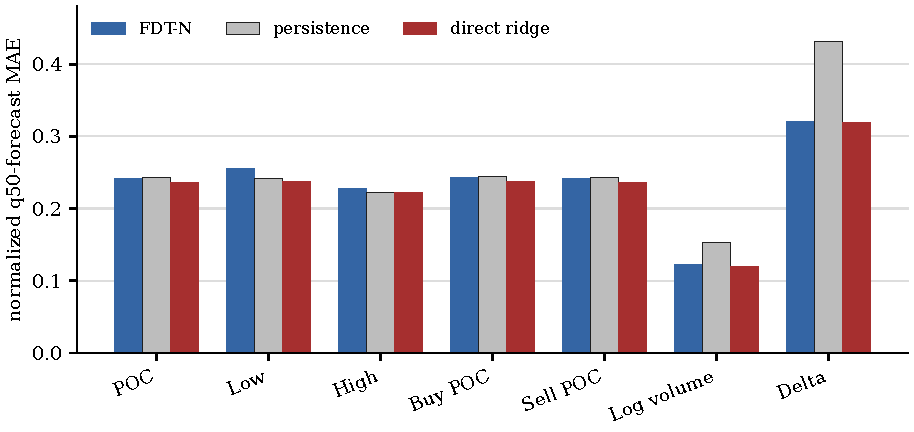
\includegraphics[width=0.92\textwidth]{assets/target-mae.pdf}
\caption{Selected-run normalized q50-forecast MAE by target. Lower is better. FDT-N's persistence
improvement is concentrated in flow variables, while direct ridge is lower for every target
aggregate.}
\label{fig:target-mae}
\end{figure}

Figure~\ref{fig:target-mae} provides the visual comparison; Table~\ref{tab:target-results} in the
appendix gives the exact values and FDT-N marginal coverage.

Pooled FDT-N MAE is 7.25\% lower than persistence and 2.68\% higher than ridge. Relative log volume
and delta fraction account for the aggregate persistence difference; across the other 40
horizon-target cells, FDT-N MAE is higher by 0.002826 on average. Ridge has lower MAE in 55 of 56
individual cells.

\subsection{Comparison by horizon}

\begin{figure}[H]
\centering
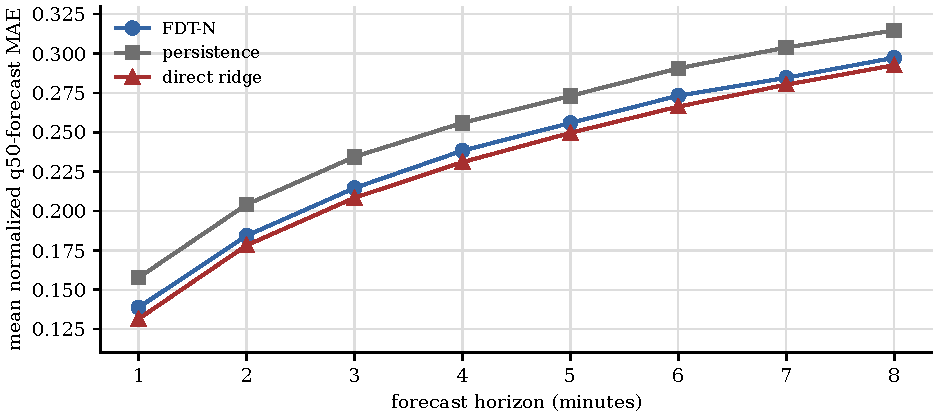
\includegraphics[width=0.90\textwidth]{assets/horizon-mae.pdf}
\caption{Q50-forecast MAE averaged over seven targets at each horizon. FDT-N lies below persistence
and above direct ridge at every horizon aggregate.}
\label{fig:horizon-mae}
\end{figure}

Figure~\ref{fig:horizon-mae} shows the horizon profile; Table~\ref{tab:horizon-results} in the
appendix lists the exact one-minute-step aggregates.

Error increases monotonically with horizon for all three methods at the aggregate level. That pattern
is descriptive; the overlapping direct targets prevent treating the eight rows as independent
replications.

\subsection{Marginal coverage}

\begin{figure}[H]
\centering
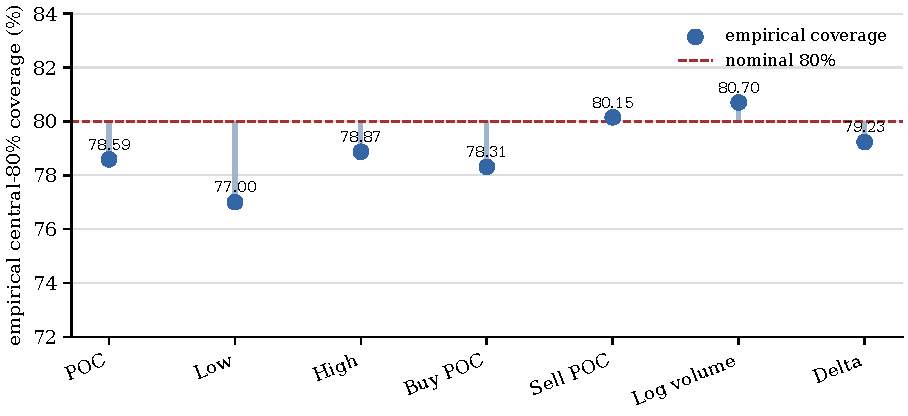
\includegraphics[width=0.88\textwidth]{assets/coverage.pdf}
\caption{Selected-run empirical central-80\% marginal coverage aggregated by target. Points show
coverage and the dashed line marks nominal 80\%.}
\label{fig:coverage}
\end{figure}

Pooled coverage is 78.98\%, target aggregates range from 77.00\% to 80.70\%, and the 56 individual
horizon-target cells range from 74.75\% to 85.66\%. These values are empirical marginal coverage on
the chronological test partition; the data split has no separate calibration partition.

\subsection{Paired resampling summaries}

\begin{figure}[H]
\centering
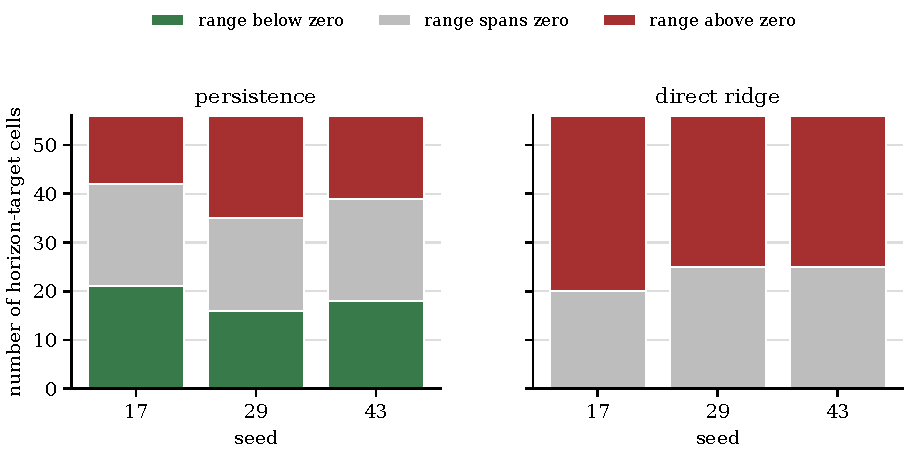
\includegraphics[width=0.84\textwidth]{assets/resampling.pdf}
\caption{Counts of 56 cellwise descriptive ranges by sign relative to zero, using the definition after
Eq.~\eqref{eq:block-bootstrap}.}
\label{fig:resampling}
\end{figure}

Figure~\ref{fig:resampling} summarizes the range signs; Table~\ref{tab:resampling} in the appendix
lists all seed-comparator counts.

Across all three seeds, the direct-ridge counts are 0 below zero, 20--25 spanning zero, and 31--36
above zero. Section~\ref{sec:resampling} defines these ranges as descriptive summaries.

\subsection{Clipping, parity, and runtime}

Price-target clipping affects approximately 1.04\%--1.17\% of observations, depending on target and
bound. Encoded row-price offset boundary saturation is 3.51\%. All reported normalized errors use the
stored clipped coordinates.

The validation-selected checkpoint is exported to ONNX. On a representative batch-one window whose
widest bar has 187 rows, ONNX Runtime differs from the PyTorch reference by maximum absolute error
$2.3842\times10^{-7}$ and mean absolute error $5.1666\times10^{-8}$, below the declared $10^{-4}$
tolerance. Across 50 isolated CPU runs, latency is 11.410/14.641/17.240 ms at p50/p95/p99. These
numbers measure isolated batch-one model execution.

\section{Interpretation}

\subsection{End-to-end behavior}

The implementation demonstrates that variable-size footprint rows can be represented without silent
compaction, pooled by a constant number of queries, combined with engineered bar features, and mapped to
ordered multi-horizon marginals in a 371,861-parameter model. The three training runs have similar
aggregate test loss and MAE. The selected export has strong numerical agreement across PyTorch and
ONNX Runtime, and its pooled central-80\% coverage is near 80\% on this test partition.

The point comparison has a consistent profile: FDT-N's pooled q50 error is lower than persistence,
principally through relative log volume and delta fraction, while direct ridge is lower for every
target aggregate, every horizon aggregate, and 55 of 56 individual cells. The paired ridge ranges are
either above zero or span zero under the sign convention in Section~\ref{sec:resampling}.

\subsection{Benchmark profile}

The latest, mean, and endpoint-difference aggregates contain substantial short-horizon location
information in this period. Each ridge cell specializes in one conditional-location estimate, whereas
FDT-N distributes 371,861 parameters across three quantiles, seven targets, and eight horizons. The
comparison therefore supplies a useful scale reference for the richer output task.

Component attribution is a separate experiment. An aggregate-only FDT-N comparison would quantify
the contribution of full rows; mean, max, one-query, and fixed-query controls would quantify pooling;
and row-only versus aggregate-only variants would quantify the fusion paths. Query interpretation
requires feature permutation, query swaps, interventions, and stability tests rather than attention
visualization alone \citep{jain2019attention}.

\subsection{Follow-up experiments}
\label{sec:follow-up}

A follow-up study can pre-register a later outer period and use anchored walk-forward development
folds. On identical windows it can compare: aggregate-only
versus full-row input; mean, max, one-query, and four-query pooling; row-only versus aggregate-only
versus gated fusion; equal versus $1/\sqrt h$ horizon weights; matched-capacity causal GRU or TCN;
train-only quantile regression and quantile trees; and a task-adapted time-series transformer where
compute and tuning budgets are comparable. A separate chronological calibration partition is needed
for any conformal or post-hoc interval adjustment.

Every target-horizon-quantile cell, clipping rate, missing-label count, and conditional slice can be
reported with a pre-specified dependence unit, multiplicity policy, and stopping rule. Cross-instrument
or cross-venue evaluation requires corresponding datasets and coordinates.

\section{Scope of the present study}
\label{sec:scope}

\paragraph{Data scope.}
The corpus covers fourteen days, one instrument, one venue, a 2.5-USDT row grid, and a maximum of 605
rows per bar. Trade-side classification, exchange corrections, row snapping, and quantity rounding
are part of the stated data-generating procedure.

\paragraph{Selection scope.}
Seed selection uses validation loss on the single chronological split. Architecture and preprocessing
belong to the same development study; an outer-period evaluation is listed as follow-up work.

\paragraph{Comparator scope.}
Persistence and ridge are q50 point baselines. The reported pinball loss and interval coverage belong
to FDT-N; matched distributional comparators and component ablations are follow-up experiments.

\paragraph{Statistical scope.}
Input windows, target horizons, and adjacent blocks overlap. The 13-block resampling ranges are
descriptive, and the three seeds summarize optimization variation on the fixed dataset and split.

\paragraph{Output scope.}
Pinball loss and coverage evaluate targetwise conditional marginals. POC sign agreement describes the
anchor-offset sign; economic or execution outcomes are outside the output contract.

\paragraph{Runtime scope.}
Parity and latency refer to the frozen batch-one model artifact. Data ingestion, bar construction,
chart rendering, and downstream decisions are separate system components.

\section{Reproducibility, availability, and declarations}

The source manifest binds the 14 official archives, while the processed dataset, three result files,
selected checkpoint, ONNX graph, metadata, and parity fixture are bound by SHA-256. Raw archives are
recoverable from Binance Data Vision. The submission bundle directly includes the executable ONNX
graph, metadata, and artifact-bound input/output fixture listed in Table~\ref{tab:hashes}; the complete
experiment lineage is recorded in \path{../research/evidence-ledger.md}.

\begin{table}[H]
\centering
\footnotesize
\caption{Packaged execution artifacts and identities. Paths are relative to this source directory.}
\label{tab:hashes}
\begin{tabularx}{\textwidth}{@{}l l X@{}}
\toprule
Artifact & Package path & SHA-256 \\
\midrule
ONNX graph & \texttt{../model/fdt-n.onnx} & \hash{adce8cd39312bf3ad1389a23ed5ca24d6f47a7f58dbb26d76ae7d54af1011af7} \\
Metadata & \texttt{../model/metadata.json} & \hash{9f998ac6b56b008ac02aaa0ed5c4f08447b1735f33027294773d9e1aa0867763} \\
Parity fixture & \texttt{../model/parity-fixture.json} & \hash{3af05175fb8c2d23f8dd33eb818c6c94afccc79135364149ef501bcf33f53160} \\
\bottomrule
\end{tabularx}
\end{table}

The recorded environment includes Python 3.12.6, PyTorch 2.5.1, NumPy 2.1.2, ONNX 1.22.0, and ONNX
Runtime 1.28.0. Result identities, seeds, configuration, parameter count, best epoch, elapsed time, and
device class are preserved in the evidence ledger.

The study uses public market-event archives and contains no personal data or human participants.
FDT-N's defined output is the marginal-quantile tensor in Table~\ref{tab:io-contract}; downstream
economic decisions are outside that interface. Dhruv Sharma is the author and performed the study,
analysis, artifact preparation, and manuscript writing.

\paragraph{Funding and competing interests.}
The artifact record identifies no external funding source or competing interest for this study.

\section{Conclusion}

FDT-N is a compact hierarchical transformer for direct marginal quantile forecasts from ragged
volume-footprint rows and engineered bar features. The mathematical construction is causal at the
bar cutoff, permutation-invariant within row sets, non-autoregressive across horizons, noncrossing
within each target, and constrained by basic price-range relationships. The input contract retains
every row for accepted bars, and the selected export passes its numerical parity tolerance.

Across three seeds, pooled normalized q50 MAE is 0.23587--0.23724. For the selected seed it is
0.235870, compared with 0.254298 for persistence and 0.229719 for direct ridge; pooled central-80\%
marginal coverage is 78.98\%. The paper's four-tensor input contract, complete layer equations,
parameter accounting, and artifact-bound forward trace make the transform from footprint rows to
$[B,8,7,3]$ outputs explicit and reproducible.

\appendix

\section{Worked input and output examples}

\subsection{Footprint arithmetic}

Consider the illustrative footprint in Table~\ref{tab:worked-footprint} with row size 0.25 price
units. These values demonstrate arithmetic only; they are not observations from the experiment.

\begin{table}[H]
\centering
\small
\caption{Illustrative completed footprint bar.}
\label{tab:worked-footprint}
\begin{tabular}{@{}rrrrrrr@{}}
\toprule
Price & Buy & Sell & Total & Delta & ZeroBid & ZeroAsk \\
\midrule
100.50 & 8 & 0 & 8 & $+8$ & 1 & 0 \\
100.25 & 32 & 6 & 38 & $+26$ & 0 & 0 \\
100.00 & 20 & 30 & 50 & $-10$ & 0 & 0 \\
99.75 & 5 & 22 & 27 & $-17$ & 0 & 0 \\
99.50 & 0 & 7 & 7 & $-7$ & 0 & 1 \\
\bottomrule
\end{tabular}
\end{table}

Summing Eq.~\eqref{eq:bar-volumes} gives $V^+=65$, $V^-=65$, $V=130$, and $\Delta=0$. The total
volumes are $(8,38,50,27,7)$, so total POC is 100.00. The largest buy volume is 32 at 100.25 and the
largest sell volume is 30 at 100.00, giving buy POC 100.25 and sell POC 100.00.

The total centroid is
\begin{align}
c&=\frac{100.50(8)+100.25(38)+100.00(50)+99.75(27)+99.50(7)}{130}\\
&=100.025.
\end{align}
Similarly, $c^+\approx100.1654$ and $c^-\approx99.8846$. For illustration, use an adjacent-larger
expansion rule for the 70\% value-area target $0.70(130)=91$. Starting at POC volume 50, compare the
adjacent 38 and 27; add 38, giving 88. Then
compare the next upper 8 with the lower 27; add 27, giving 115. The resulting contiguous value area
is 99.75--100.25.

For the 100.25 row, the offset is one row increment and
\begin{equation}
\frac{v^+}{V}=\frac{32}{130}=0.2462,\quad
\frac{v^-}{V}=\frac{6}{130}=0.0462,\quad
\frac{v}{V}=\frac{38}{130}=0.2923,\quad
\frac{\Delta}{V}=\frac{26}{130}=0.2000.
\end{equation}
If the bar POC is 100.00, the first row feature in Eq.~\eqref{eq:row-features} is
$1/32=0.03125$, not the unscaled one-row offset.

Suppose an illustrative one-step q50 predicts normalized POC offset $1/64$, low $-1/64$, high
$4/64$, buy POC $1/64$, sell POC 0, normalized relative log volume 0.05, and delta fraction 0.10.
The inverse prices are 100.25, 99.75, 101.00, 100.25, and 100.00. If the context reference satisfies
$\exp(\widetilde\ell_t)=101$, then
\begin{equation}
\widehat V=\exp(\widetilde\ell_t+4(0.05))-1=101e^{0.2}-1\approx122.36.
\end{equation}
Multiplying this q50 volume plug-in by the q50 delta fraction gives 12.24, but that product is not the
q50 of delta volume because quantiles do not generally commute with products of dependent random
variables.

Finally, suppose illustrative POC q10/q50/q90 offsets are $(-1,1,3)$ row increments and the
realization is 2. By Eq.~\eqref{eq:pinball}, the losses are
\begin{equation}
0.1(2-(-1))=0.3,\qquad
0.5(2-1)=0.5,\qquad
0.1(3-2)=0.1,
\end{equation}
whose unweighted mean is 0.3 row increment.

\subsection{Artifact-bound forward pass}

This example is read directly from \path{../model/parity-fixture.json} and executed by the packaged
\path{../model/fdt-n.onnx}. The deterministic fixture rule chooses the earliest window whose padded
row width reaches the corpus p95, so selection depends on input width. Its last context bar starts at
2024-01-10 19:13:00 UTC and the first forecast cutoff is 19:14:00 UTC. The last-context POC anchor is
46,465 USDT, the row size is 2.5 USDT, and the context log-volume reference is
$\widetilde\ell_t=11.59615697$.

\begin{table}[H]
\centering
\small
\caption{The four actual fixture inputs. $N=187$ is the widest bar in this window; valid row counts
range from 8 to 187 and padding is identified only by the boolean mask.}
\label{tab:fixture-inputs}
\begin{tabular}{@{}lll@{}}
\toprule
Tensor & Shape & Content \\
\midrule
\texttt{row\_features} & $[1,64,187,11]$ & encoded rows, oldest bar to newest bar \\
\texttt{row\_mask} & $[1,64,187]$ & observed-row indicators; last bar has 56 rows \\
\texttt{bar\_features} & $[1,64,23]$ & aggregate history in schema order \\
\texttt{bar\_mask} & $[1,64]$ & 64 valid completed bars \\
\bottomrule
\end{tabular}
\end{table}

Table~\ref{tab:fixture-inputs} makes the dynamic row width and both masks concrete for this window.
Table~\ref{tab:fixture-trace} records actual intermediate tensors from that pass, restoring the batch
axis to the row-set summary. ``First four'' means the first four values in deterministic flattened
storage; the statistic is RMS except for the sigmoid gate, for which the mean is more interpretable.

\begin{table}[H]
\centering
\footnotesize
\caption{Artifact-bound processing trace.}
\label{tab:fixture-trace}
\begin{tabular}{@{}l l r l@{}}
\toprule
Stage & Shape & Statistic & First four values \\
\midrule
Row-set summary $A$ & $[1,64,64]$ & 0.982983 & 0.818572, 1.133166, $-0.201165$, $-0.125622$ \\
Bar summary & $[1,64,64]$ & 1.008219 & $-0.568567$, 0.931088, $-0.373822$, $-2.358358$ \\
Fusion gate & $[1,64,64]$ & 0.527938 & 0.508116, 0.125989, 0.452889, 0.394906 \\
Fused history $U$ & $[1,64,64]$ & 1.013353 & 0.188924, 1.828844, 0.049782, $-1.720833$ \\
Temporal memory $\mathcal H$ & $[1,64,64]$ & 1.004026 & 0.224272, 2.108123, $-0.058805$, $-1.318258$ \\
Decoder $D^{(2)}$ & $[1,8,64]$ & 1.991881 & $-1.489616$, $-0.704202$, 0.551906, 2.596395 \\
Affine head $R_{\mathrm{flat}}$ (pre-reshape) & $[1,8,21]$ & 0.838586 & $-0.191553$, $-0.529968$, $-0.584842$, 0.546425 \\
\bottomrule
\end{tabular}
\end{table}

For horizon one, Table~\ref{tab:fixture-output} shows the raw head triples and the actual ONNX return.
For example, POC uses
\begin{equation}
q_{.1}=-0.191553-\softplus(-0.529968)-10^{-4}=-0.654521,
\end{equation}
with q50 equal to the center and q90 formed by the upper softplus spread. Low and side-POC values are
then clamped by Eq.~\eqref{eq:physical-constraints}; delta values pass through $\tanh$.

\begin{table}[H]
\centering
\footnotesize
\caption{Actual horizon-one raw head and constrained normalized output.}
\label{tab:fixture-output}
\begin{tabular}{@{}l rrr rrr@{}}
\toprule
& \multicolumn{3}{c}{Raw $(c,s^-,s^+)$} & \multicolumn{3}{c}{Returned (q10, q50, q90)} \\
Target & $c$ & $s^-$ & $s^+$ & q10 & q50 & q90 \\
\midrule
POC & $-0.191553$ & $-0.529968$ & $-0.584842$ & $-0.654521$ & $-0.191553$ & 0.251432 \\
Low & 0.546425 & $-1.126999$ & 0.763642 & $-0.654521$ & $-0.191553$ & 0.251432 \\
High & 0.054772 & $-1.039371$ & $-0.635295$ & $-0.248153$ & 0.054772 & 0.479995 \\
Buy POC & $-0.810497$ & 0.995014 & $-0.557284$ & $-0.654521$ & $-0.191553$ & 0.251432 \\
Sell POC & $-0.887576$ & 1.075034 & 0.601971 & $-0.654521$ & $-0.191553$ & 0.251432 \\
Log volume & $-0.148085$ & $-2.036494$ & $-1.665860$ & $-0.270832$ & $-0.148085$ & 0.025151 \\
Delta fraction & 0.050435 & $-1.225202$ & $-1.040504$ & $-0.204256$ & 0.050392 & 0.339090 \\
\bottomrule
\end{tabular}
\end{table}

The price inverse is $46{,}465+2.5(64)q$, and scaled volume is divided by the recorded quantity scale
1,000 to obtain BTC. The returned physical marginals are therefore
\begin{center}
\begin{tabular}{@{}lrrr@{}}
\toprule
Target & q10 & q50 & q90 \\
\midrule
POC / low / buy POC / sell POC (USDT) & 46,360.28 & 46,434.35 & 46,505.23 \\
High (USDT) & 46,425.30 & 46,473.76 & 46,541.80 \\
Volume (BTC) & 36.783 & 60.102 & 120.181 \\
Delta fraction & $-0.204256$ & 0.050392 & 0.339090 \\
\bottomrule
\end{tabular}
\end{center}
PyTorch and ONNX Runtime return the same full $[1,8,7,3]$ tensor within maximum absolute difference
$2.3842\times10^{-7}$ and mean absolute difference $5.1666\times10^{-8}$.

\section{Detailed benchmark tables}

\begin{table}[H]
\centering
\small
\caption{Selected-run target aggregates. Coverage is empirical marginal q10--q90 coverage for
FDT-N; point baselines have no interval.}
\label{tab:target-results}
\begin{tabular}{@{}lrrrr@{}}
\toprule
Target & FDT-N MAE & Persistence MAE & Ridge MAE & FDT-N coverage \\
\midrule
POC offset & 0.2414 & 0.2432 & 0.2357 & 78.59\% \\
Low offset & 0.2552 & 0.2423 & 0.2371 & 77.00\% \\
High offset & 0.2272 & 0.2221 & 0.2225 & 78.87\% \\
Buy-POC offset & 0.2431 & 0.2442 & 0.2374 & 78.31\% \\
Sell-POC offset & 0.2415 & 0.2426 & 0.2359 & 80.15\% \\
Relative log volume & 0.1219 & 0.1536 & 0.1198 & 80.70\% \\
Delta fraction & 0.3207 & 0.4321 & 0.3197 & 79.23\% \\
\midrule
Pooled & 0.235870 & 0.254298 & 0.229719 & 78.98\% \\
\bottomrule
\end{tabular}
\end{table}

\begin{table}[H]
\centering
\small
\caption{Selected-run horizon aggregates. Horizons are one-minute steps.}
\label{tab:horizon-results}
\begin{tabular}{@{}crrrr@{}}
\toprule
Horizon & FDT-N MAE & Persistence MAE & Ridge MAE & FDT-N coverage \\
\midrule
1 & 0.1388 & 0.1577 & 0.1315 & 83.41\% \\
2 & 0.1843 & 0.2041 & 0.1782 & 79.45\% \\
3 & 0.2146 & 0.2344 & 0.2084 & 78.55\% \\
4 & 0.2383 & 0.2560 & 0.2310 & 78.80\% \\
5 & 0.2559 & 0.2731 & 0.2496 & 77.44\% \\
6 & 0.2732 & 0.2906 & 0.2663 & 77.64\% \\
7 & 0.2846 & 0.3038 & 0.2802 & 78.07\% \\
8 & 0.2973 & 0.3147 & 0.2926 & 78.45\% \\
\bottomrule
\end{tabular}
\end{table}

\begin{table}[H]
\centering
\small
\caption{Cell counts under paired four-hour block resampling.}
\label{tab:resampling}
\begin{tabular}{@{}clrrr@{}}
\toprule
Seed & Comparator & Below zero & Spans zero & Above zero \\
\midrule
17 & Persistence & 21 & 21 & 14 \\
29 & Persistence & 16 & 19 & 21 \\
43 & Persistence & 18 & 21 & 17 \\
17 & Direct ridge & 0 & 20 & 36 \\
29 & Direct ridge & 0 & 25 & 31 \\
43 & Direct ridge & 0 & 25 & 31 \\
\bottomrule
\end{tabular}
\end{table}

\section{Notation and dimensional reference}

Table~\ref{tab:notation} collects the symbols used throughout the derivation.

\begin{longtable}{@{}p{0.18\textwidth}p{0.74\textwidth}@{}}
\caption{Principal notation.}\label{tab:notation}\\
\toprule
Symbol & Meaning \\
\midrule
\endfirsthead
\toprule
Symbol & Meaning \\
\midrule
\endhead
$t,j,h,k,\tau$ & bar, row, forecast horizon, target, and quantile indices \\
$L,H,K,Q$ & 64 history bars, 8 horizons, 7 targets, and 3 quantile levels \\
$p,v^+,v^-,v,\Delta$ & row price, buy volume, sell volume, total volume, and signed delta \\
$R_t,n_t$ & complete accepted row set for bar $t$ and its variable cardinality \\
$B_t=(R_t,b_t)$ & completed footprint bar with row set and 23-vector aggregates \\
$\delta_p,S_g,S_p,S_v$ & 2.5-USDT row size; 32-row input-gap scale; 64-row target scale; log-volume scale 4 \\
$d,A,d_h,K_q$ & model width 64, 4 heads, head width 16, and 4 row queries \\
$m_{bhk}$ & target-validity mask; padding has a separate row-attention mask \\
$q_{i,.1},q_{i,.5},q_{i,.9}$ & predicted marginal q10, q50, and q90 in normalized target coordinates \\
$\rho_\tau$ & pinball loss at quantile level $\tau$ \\
\bottomrule
\end{longtable}

\bibliographystyle{plainnat}
\bibliography{references}

\end{document}
